% !TEX root=../MA119-Main.tex

\begin{tcolorbox}[colback=white,colframe=cyan, title filled=false, coltitle=cyan, enhanced, attach boxed title to top center={yshift=-3mm,yshifttext=-1mm}, fonttitle=\bfseries, boxed title style={size=small,colback=white}, before upper={\parindent15pt},
title={The slope-intercept form equation}]
The slope of a line measures the steepness, in other words, ``rise'' over ``run'', or rate of change,  of the line. Using the rectangular coordinate  system, the \dfn{slope} $m$ of a line is defined as\\ 
\centerline{$m=\dfrac{y_2-y_1}{x_2-x_1}=\dfrac{\textup{rise}}{\textup{run}}$,}\\
 where $(x_1, y_1)$ and $(x_2, y_2)$ are any two distinct points on the line. If the line intersects the $y$-axis at the point $(0, b)$, then a point $(x, y)$ is on the line if and only if\\ \centerline{$y=mx+b$.}\\ This equation is called the \dfn{slope-intercept form} of the line.
\end{tcolorbox}


%
%\begin{tcolorbox}[colback=white,colframe=cyan, title filled=false, coltitle=cyan, enhanced, attach boxed title to top center={yshift=-3mm,yshifttext=-1mm}, fonttitle=\bfseries, boxed title style={size=small,colback=white}, before upper={\parindent15pt},
%title={Linear Function}]
%\begin{multicols}{2}
%A \dfn{linear function} is a function whose graph is a line. Using function notation, a linear functions can be written in the slope-intercept form of a line:\\
%\centerline{$f(x) = mx + b$,}\\
%where $m$ is the slope and $(0, b)$ is the $y$-intercept.
%\columnbreak
%
%Note if a function $f(x)$ is a linear function, then\\ \centerline{$b=f(0)$}\\ and the slope\\
%\centerline{$m=\dfrac{f(x_2)-f(x_1)}{x_2-x_1}=\dfrac{\text{change in output}}{\text{change in input}}$.}\\
%%or informally, \\
%%\centerline{$m=\dfrac{\text{change in output}}{\text{change in input}}.%$} 
%
%\end{multicols}
%\end{tcolorbox}



\begin{tcolorbox}[title={How to write an equation for a line?}]

\begin{example}
 A line passes through two points $(2, 5)$ and $(-1,2)$. Find an equation for the line in slope-intercept form.
\begin{enumerate}[label={\textbf{Step \arabic*.}~}, itemsep=0em, itemindent=1ex]
\item Find the slope $m$: $m=\frac{5-2}{2-(-1)}=\frac{3}{3}=1$. 
\item 
To find $b$, plug $x=2$ into the slope-intercept form $y=x+b$ and then solve for $b$: \vspace*{-0.5em}
\[\begin{split}
5&=2+b\\
5+(-2)&=2+(-2)+b\\
3&=b
\end{split}\]
\vspace*{-2em}
\item The slope-intercept form equation of the line is $y=x+3$.
 \end{enumerate}
\end{example}
\end{tcolorbox}



\begin{tcolorbox}[title={Sketch the graph of a linear function via plotting points}]
\begin{example}
Sketch the graph of the line defined by the equation $y=-\frac12 x + 1$.
\vspace*{-1em}
\begin{multicols}{2}
\textbf{Method 1: Get points $(x, y)$ by choosing  $x$ and finding $y$.}
% \vspace*{-1em}
\begin{enumerate}[label={\textbf{Step \arabic*.}~}, itemsep=0em]
\item Choose two or more input values, e.g. $x=0$ and $x=2$.
\item Find  $y$: $y_1=-\frac12\cdot 0+1=1$ and $y_2=-\frac12\cdot 2+1=0$.
\item Plot the points $(0, 1)$ and $(2, 0)$ and draw a line through them.
\end{enumerate}

\columnbreak


\textbf{Method 2: Get points the slope and $y$-intercept.}
% \vspace*{-1em}
\begin{enumerate}[label={\textbf{Step \arabic*.}~}, itemsep=0em]
\item Plot the $y$-intercept $(0, 1)$.
\item Use $\frac{\textup{rise}}{\textup{run}}=-\frac{1}{2}$ to get one or more points, e.g, we will get $(-2, 2)$ by taking $\text{rise}=1$ and $\text{run}=-2$, i.e. move up $1$ unit, then move to the right $2$ units.  
\item Plot the points $(0, 1)$ and $(-2, 2)$ and draw a line through them.
\end{enumerate}
\end{multicols}

\vspace{1em}
\begin{multicols}{2}
\begin{center}
\begin{tikzpicture}[scale=0.7, every node/.style={scale=0.7}]
 \begin{axis}[grid=both, unit vector ratio=1 1 1, ymin=-0.5,ymax=2.5,xmax=3,xmin=-3.1,xtick={-3,-2,...,3},ytick={-3,-2,...,4},minor tick num=1,axis lines = middle,xlabel=$x$,ylabel=$y$, 
x tick label style={yshift=0.25ex,font={\small}}, y tick label style={xshift=0ex, font={\small}}, label style ={at={(ticklabel cs:1.1)}, font={\small}}
]
 \addplot[thick, samples=100,domain=-3:3, name path=A, stealth-stealth]   {-1/2*x+1};           
  \node[draw,shape=circle, minimum size=2mm,inner sep=0pt,outer sep=0pt, fill=black] at (0,1) {}; 
  \node[draw,shape=circle, minimum size=2mm,inner sep=0pt,outer sep=0pt, fill=black] at (2,0) {};                
  \end{axis}
\end{tikzpicture}
\end{center}

\columnbreak

\begin{center}
\begin{tikzpicture}[scale=0.7, every node/.style={scale=0.7}]
 \begin{axis}[grid=both, unit vector ratio=1 1 1, ymin=-0.5,ymax=2.5,xmax=3,xmin=-3,xtick={-3,-2,...,3},ytick={-3,-2,...,4},minor tick num=1,axis lines = middle,xlabel=$x$,ylabel=$y$, 
x tick label style={yshift=0.25ex,font={\small}}, y tick label style={xshift=0ex, font={\small}}, label style ={at={(ticklabel cs:1.1)}, font={\small}}
]
 \addplot[thick, samples=100,domain=-3:3, name path=A, stealth-stealth]   {-1/2*x+1};           
  \node[draw,shape=circle, minimum size=2mm,inner sep=0pt,outer sep=0pt, fill=black] at (0,1) {};  
  \node[draw,shape=circle, minimum size=2mm,inner sep=0pt,outer sep=0pt, fill=black] at (-2,2) {};   
  \addplot[blue, draw, -stealth] (0, 1)--(0,2) node[midway, xshift=1.5em] {rise=1}; 
  \addplot[red, draw, -stealth] (0, 2)--(-2,2) node[midway, yshift=0.5em] {run=-2};          
  \end{axis}
\end{tikzpicture}
\end{center}

\end{multicols}
\end{example}
\end{tcolorbox}





\newpage

\begin{multicols}{2}
\begin{exercise}
Finding the slope of a line passing through $(3,5)$ and $(-1, 1)$.
\end{exercise}

\columnbreak
\begin{exercise}
Find the slope-intercept form equation of a line passing through $(6, 3)$ and $(2, 5)$.
\end{exercise}
\end{multicols}
\vfill


\begin{exercise}Suppose the line $L_1$ passes through $(-2, -4)$ and $(0, 2)$ and the line $L_2$ passes through $(0, 2)$ and $(2, 8)$. 
Determine if they are defined by the same equation. Explain your answer.  
\end{exercise}
\vfill

\begin{exercise}
Graph the line $y=-x + 1$.


\begin{multicols}{2}
\begin{center}
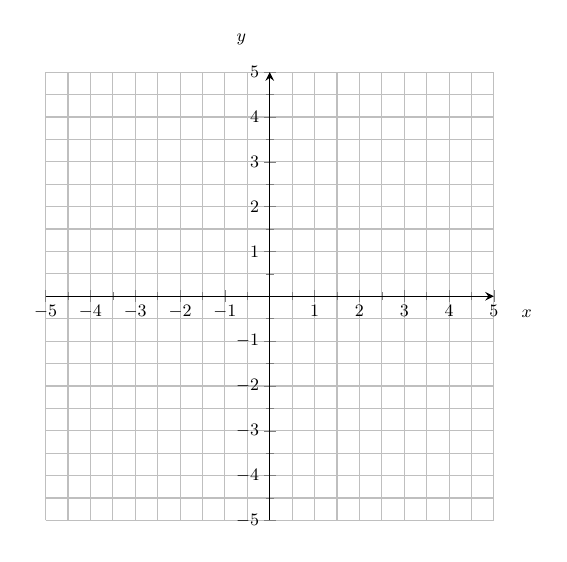
\begin{tikzpicture}[scale=1, every node/.style={scale=0.7}]
 \begin{axis}[grid=both, unit vector ratio=1 1 1, ymin=-5,ymax=5,xmax=5,xmin=-5,xtick={-10,-9,...,9,10},ytick={-10,-9,...,9,10},minor tick num=1,axis lines = middle,xlabel=$x$,ylabel=$y$, 
x tick label style={yshift=0.5ex,font={\small}}, y tick label style={xshift=0.25ex, font={\small}}, label style ={at={(ticklabel cs:1.1)}, font={\small}}
]
% \addplot[thick, samples=100,domain=-3:3, name path=A, stealth-stealth]   {-1/2*x+1};           
%  \node[draw,shape=circle, minimum size=2mm,inner sep=0pt,outer sep=0pt, fill=black] at (0,1) {}; 
%  \node[draw,shape=circle, minimum size=2mm,inner sep=0pt,outer sep=0pt, fill=black] at (2,0) {};                
  \end{axis}
\end{tikzpicture}
\end{center}

\columnbreak

\begin{center}
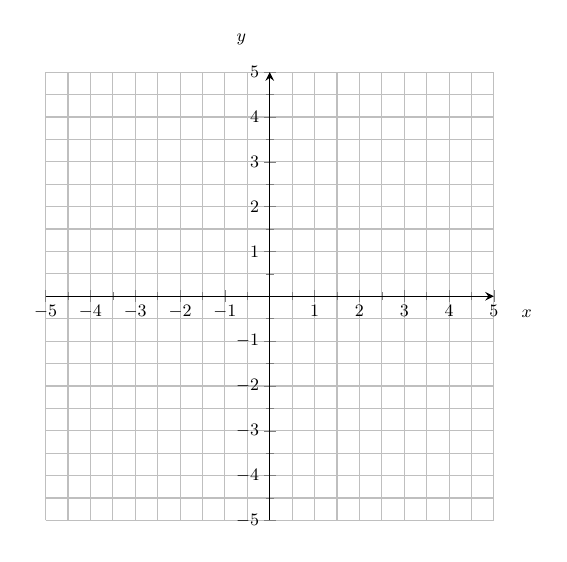
\begin{tikzpicture}[scale=1, every node/.style={scale=0.7}]
 \begin{axis}[grid=both, unit vector ratio=1 1 1, ymin=-5,ymax=5,xmax=5,xmin=-5,xtick={-10,-9,...,9,10},ytick={-10,-9,...,9,10},minor tick num=1,axis lines = middle,xlabel=$x$,ylabel=$y$, 
x tick label style={yshift=0.5ex,font={\small}}, y tick label style={xshift=0.25ex, font={\small}}, label style ={at={(ticklabel cs:1.1)}, font={\small}}
]
% \addplot[thick, samples=100,domain=-3:3, name path=A, stealth-stealth]   {-1/2*x+1};           
%  \node[draw,shape=circle, minimum size=2mm,inner sep=0pt,outer sep=0pt, fill=black] at (0,1) {};  
%  \node[draw,shape=circle, minimum size=2mm,inner sep=0pt,outer sep=0pt, fill=black] at (-2,2) {};   
%  \addplot[blue, draw, -stealth] (0, 1)--(0,2) node[midway, xshift=1.5em] {rise=1}; 
%  \addplot[red, draw, -stealth] (0, 2)--(-2,2) node[midway, yshift=0.5em] {run=-2};          
  \end{axis}
\end{tikzpicture}
\end{center}

\end{multicols}

\end{exercise}

\vspace{1cm}

%\vspace{\fill}
\hrule

\hfill

\raisebox{0.5em}{\rotatebox{\rotationdegree}{
\begin{enumerate*}[label={(\arabic*)~}]
\item  $m=1$\quad\quad
\item $y=-\frac12x+6$.\quad\quad
\item Yes. Because $y=3x + 2$ and $y=3x+2$.
\end{enumerate*}
}}%\fi


